\beginsong{Danke}[
    wuw={Martin Gotthard Schneider}, 
    jahr={1961},
    pfii={130},
    eg={334},
]

\beginverse
\[C]Danke für diesen \[F]guten \[G]Morgen, \[C]danke für jeden \[F]neuen \[G]Tag.
\[C]Danke, dass ich all \[F]meine S\[G]orgen \[F]auf Dich \[G]werfen \[C]mag.
\endverse

%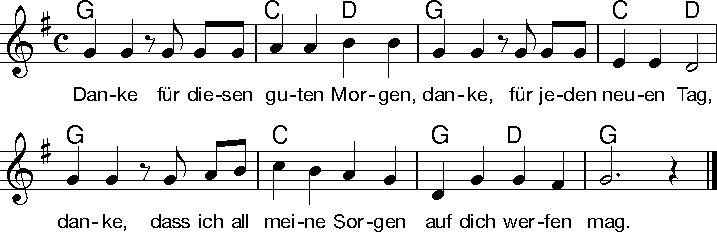
\includegraphics[draft=false, width=1\textwidth]{Noten/Lied107.pdf}

\beginverse
\[C]Danke für meine \[F]guten \[G]Freunde, \[C]danke, oh Herr, für \[F]jeder\[G]mann,
\[C]danke, wenn auch dem \[F]größten \[G]Feinde \[F]Ich ver\[G]zeihen \[C]kann.
\endverse

\beginverse
^Danke für meine ^Arbeits^stelle, ^danke für jedes ^kleine ^Glück,
^danke für alles ^frohe ^Helle ^und für ^die Mu^sik.
\endverse

\beginverse
^Danke für manche ^Traurig^keiten, ^danke für jedes ^gute ^Wort,
^danke, dass deine ^Hand mich ^leiten ^will an ^jeden ^Ort.
\endverse

\beginverse
^Danke, dass ich dein ^Wort ver^stehe, ^danke, dass deinen ^Geist du ^gibst,
^danke, dass in der ^Fern' und ^Nähe ^du die ^Menschen ^liebst
\endverse

\beginverse
^Danke, ^ ^ ^danke, ^ ^
^danke, ^ ^ ^danke. ^ ^
\endverse

\endsong
